
\chapter{Data set analysis and definition of variables}



\section{Introduction to the data set}

We used the MJFF Levadopa dataset. Subjects in this data were furnished with three or eight sensors, with subjects wearing a GeneActiv on the wrist of the most severely affected limb, a Pebble smartwatch on the wrist of the least affected limb, and a Samsung Galaxy Mini smartphone at the waist. These sensors were worn off for the study duration, and subjects recruited from the Boston study site were equipped with five sensors (Shimmer 3), one for each limb and one for the waist. The Shimmer sensors corresponded to the left ankle, right ankle, left wrist, right wrist, and back. \cite{MJFF}
\\ \hspace*{\fill} \\
\begin{figure}[htbp]
    \centering
    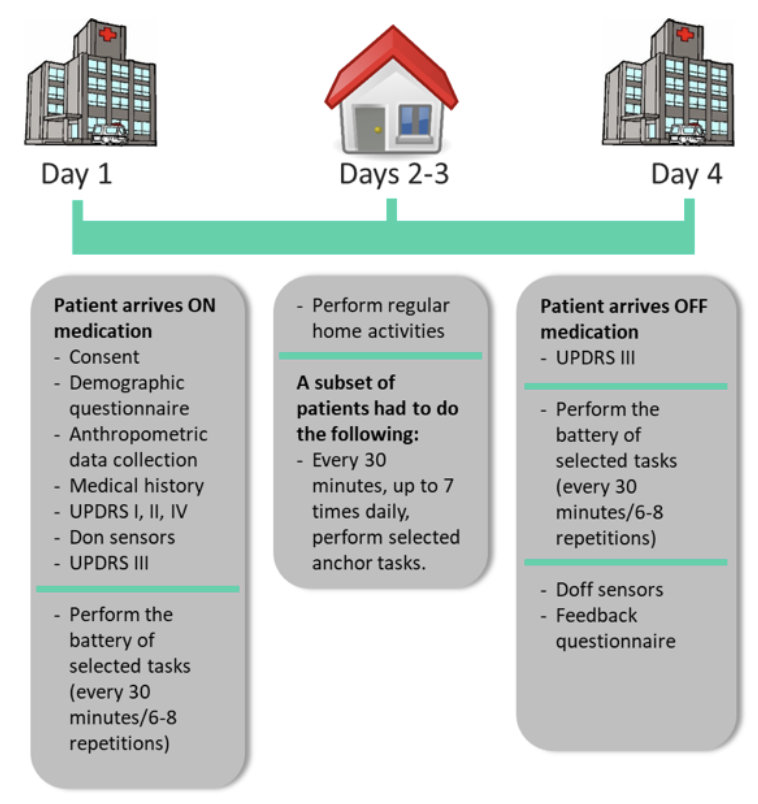
\includegraphics[width=9cm]{report/pics/Day.png}
    \caption{The process by which the dataset was collected \cite{MJFF}}
    \label{fig:my_label}
\end{figure}

\begin{figure}[htbp]
    \centering
    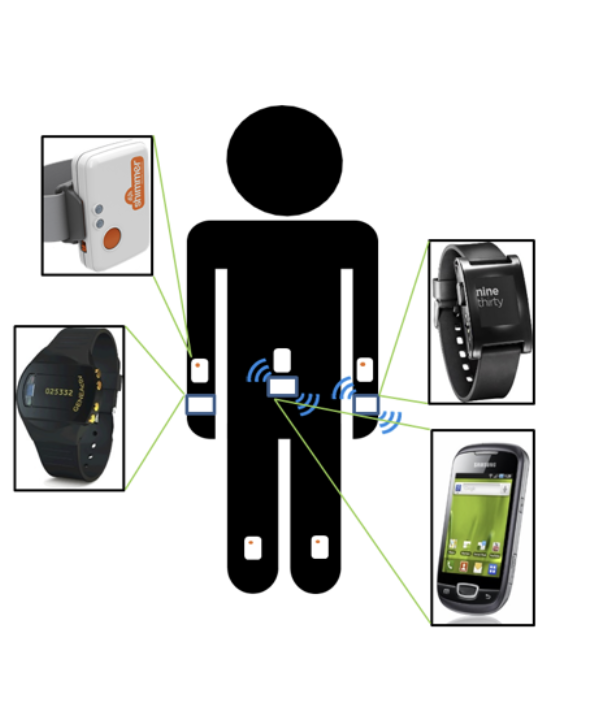
\includegraphics[width=7cm]{report/pics/Sensor.png}
    \caption{About the Sensor Wearing Figure, the Shimmer Sensor is worn on five different parts of the body. \cite{MJFF}}
    \label{fig:my_label}
\end{figure}



A total of 19 subjects, each subject was collected four days of sensor data. On the first day, they had several motor tasks, including standing, walking in a straight line for the 30s, walking in a straight line for 30s while counting backward, walking up and downstairs, walking through a narrow corridor, finger to nose for 15s (twice per arm), regarding other activities: alternating hand movements for 15s (twice for each arm), drawing, typing on the keyboard for the 30s, opening and pouring bottles (three times), arranging pieces of paper in a folder (twice), assembling nuts and bolts for 30s, folding a towel three times and then sitting. On the second and third day, the test subjects wear the sensors at home and record their usual activities and motor tasks, and finally, on the fourth day, the subjects perform the activities from the first day. For this dataset, we will use Shimmer sensor data and datasets to assess the severity of symptoms of Parkinson's disease. Shimmer sensor data is collected in 3 dimensions, per site $(x, y, z)$, with a total of 5 Shimmer sensors corresponding to 15 different datasets being collected simultaneously. The Shimmer sensor (IMU Sensor) collects IMU data as a variable over four consecutive days. The sensor also records data on the abnormal activity of the test subject's Parkinson's disease over the four days. The accelerations in the X, Y, and Z axes collected by the sensor allow us to determine abnormal activity in Parkinson's patients. For example, when a Parkinson's patient has hand tremors, the sensor worn on the hand can record accelerations that are not consistent with regular activity. The dataset also includes ratings for Parkinson's disease (Bradykinesia, dyskinesia, tremor), each with a 0-4, 0 is no symptom occurrence, and 4 is the most severe occurrence of the symptom. So the IMU data collected for abnormal Parkinson's activity can correspond to the rating for each condition. \cite{MJFF}
\\



\begin{figure}[htbp]
    \centering
    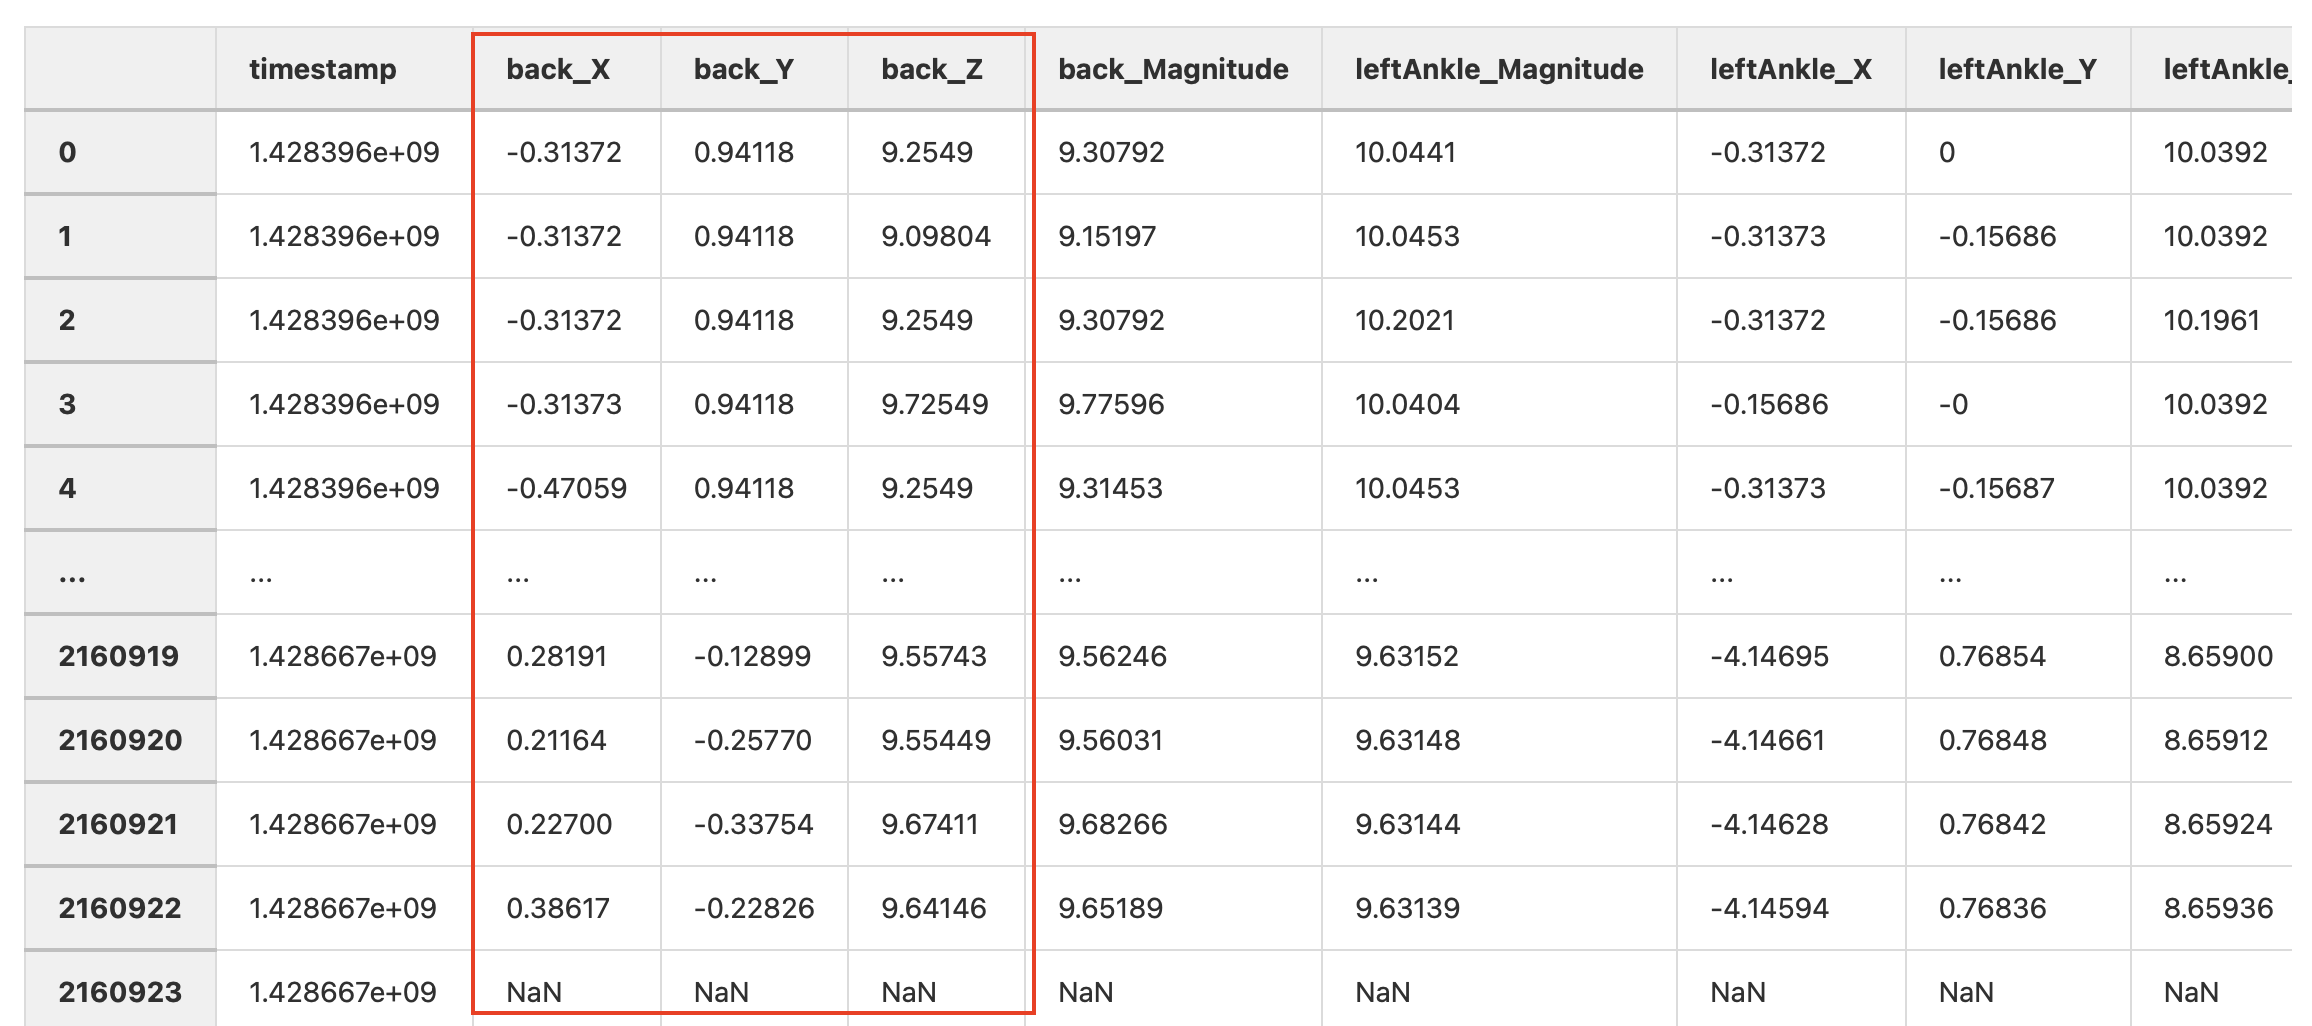
\includegraphics[width=13cm]{report/pics/X.png}
     \caption{IMU acceleration collected from Shimmer sensors worn by Parkinson's patients \cite{MJFF}}
    \label{fig:my_label}
\end{figure}


\begin{figure}[htbp]
    \centering
    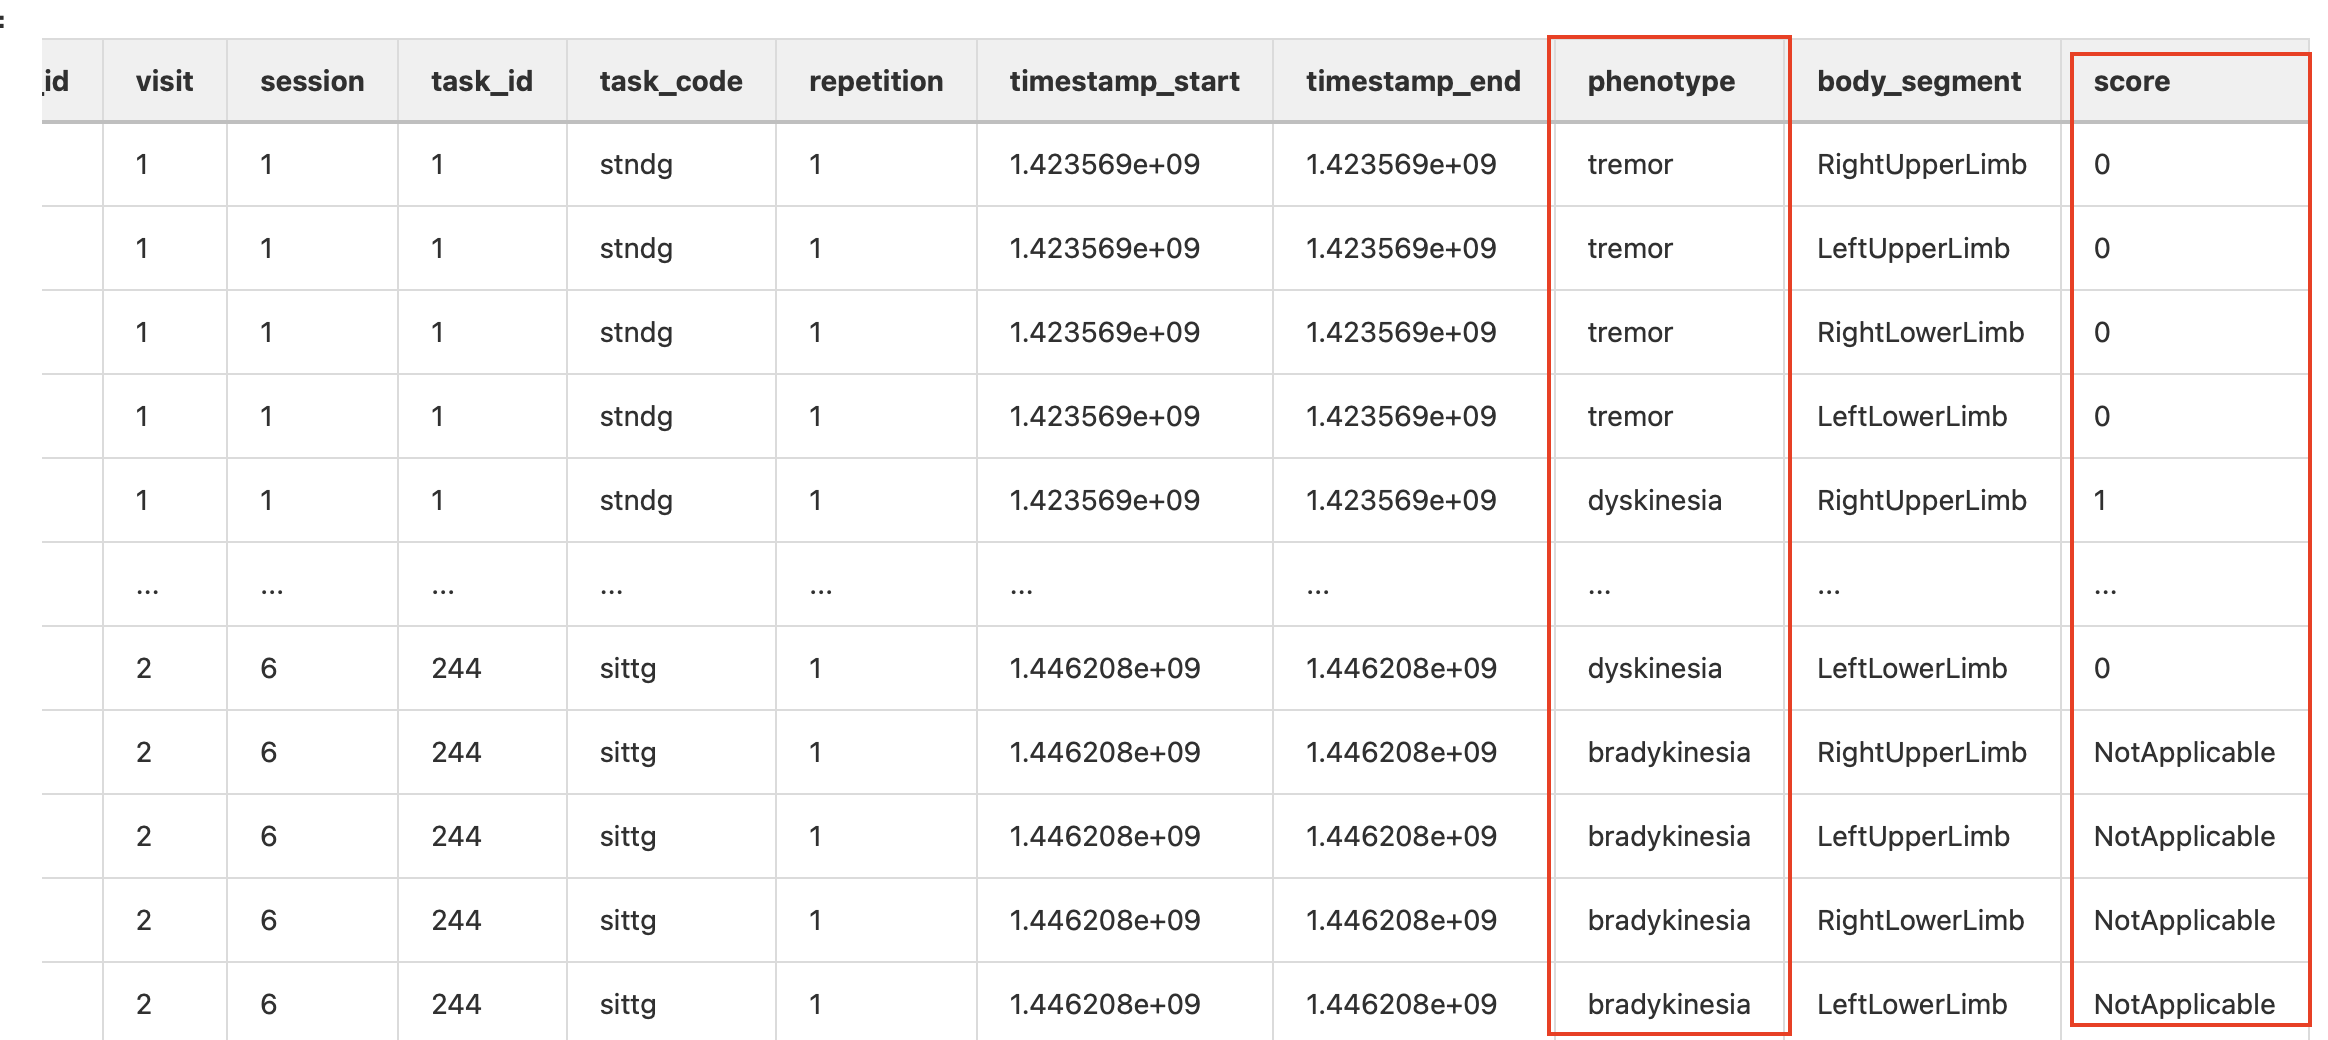
\includegraphics[width=13cm]{report/pics/Y.png}
    \caption{The dataset is rated for Parkinson's disease, with each phenotype corresponding to a score. There will also be some non-applicable data. \cite{MJFF}}
    \label{fig:my_label}
\end{figure}











\subsection{Visualization Analysis}
When visualized, the IMU data helps us understand the data better. Figure 5.5 demonstrates that five different sensors recorded acceleration during dyskinesia, which lasted 32.98 seconds.
\begin{figure}[htbp]
    \centering
    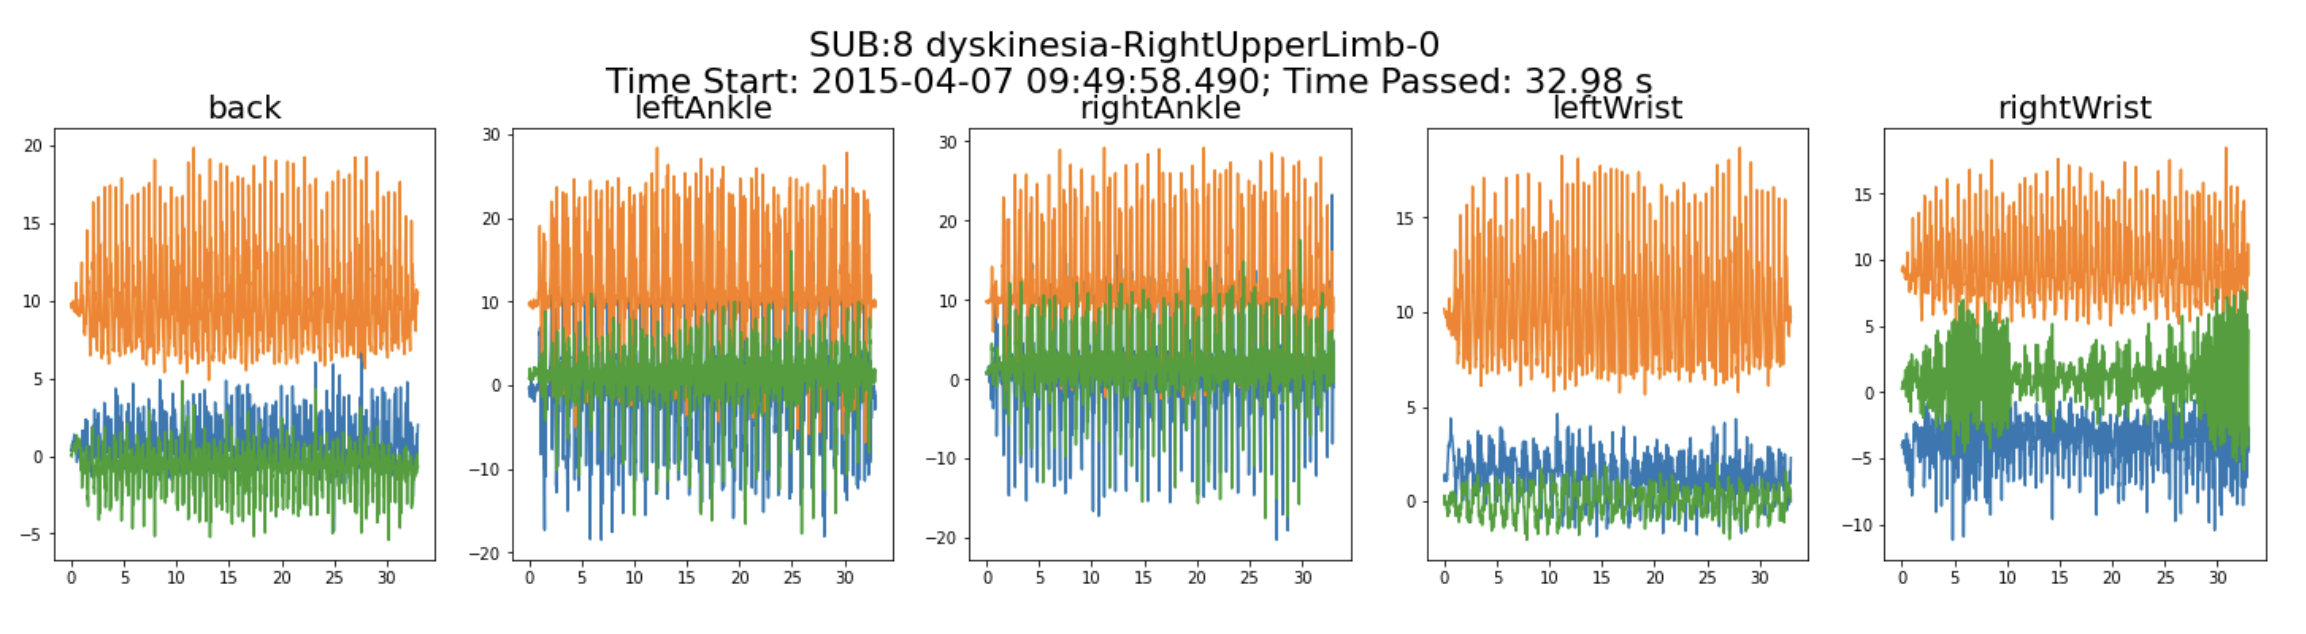
\includegraphics[width=13cm]{report/pics/dyskinesia-RightUpperLimb.png}
    \caption{Acceleration collected by 5 Shimmer sensors in 32.98 seconds accompanied by dyskinesia \cite{MJFF}}
    \label{fig:my_label}
\end{figure}\\

Figure 5.6 shows the percentage of scores for the tremor condition in 34 hours, 52 minutes, and 17 seconds, and we can see that 0 scores account for 72.75\% of the scores. The scores of dyskinesia and bradykinesia are also shown. In bradykinesia, the percentage of "none" and "yes" is significant. Therefore, it cannot be used for motor retardation disorders when quantifying information loss. There is also the proportion of simultaneously rated bradykinesia, again with "0" occupying most of the time and rating "4" occupying very little of the time. Most of the time, patients with Parkinson's disease are 'on' state, so the severity of Parkinson's impairment is 0. The ratings '1-4', on the other hand, indicate the severity of Parkinson's impairment from mild to severe.

\begin{figure}[htbp]
    \centering
    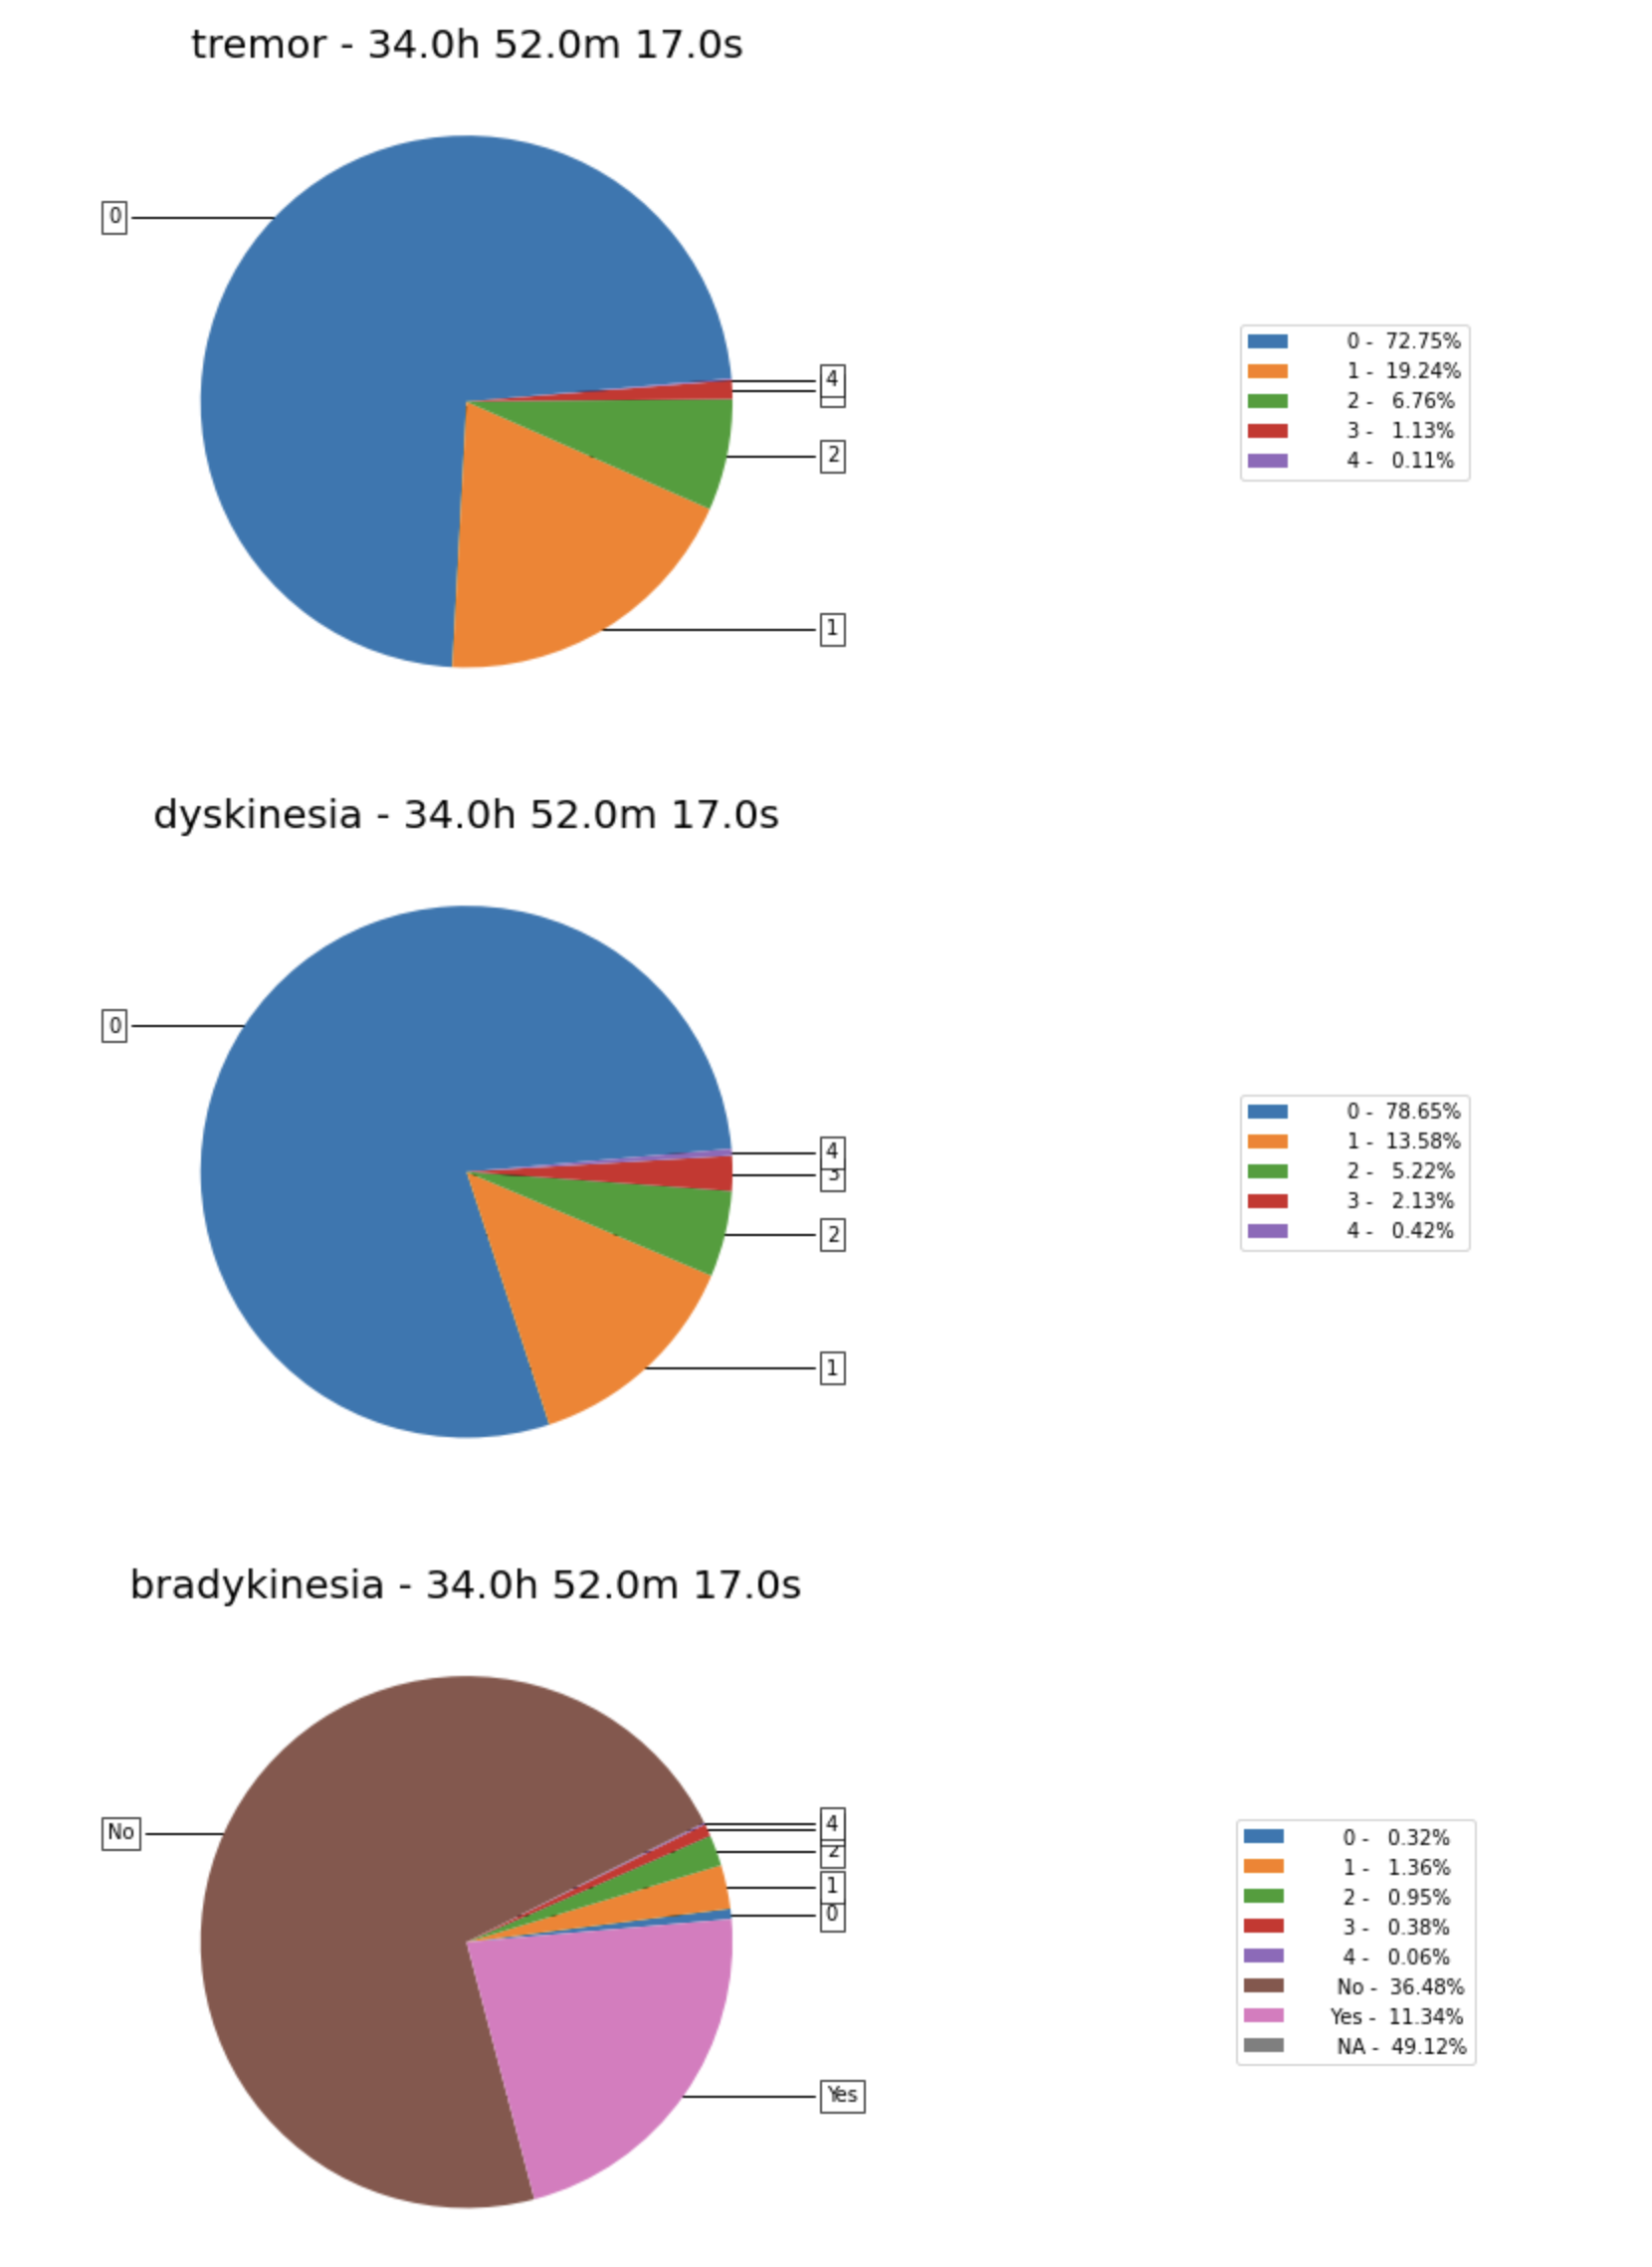
\includegraphics[width=12cm]{report/pics/PD.png}
    \caption{Diagram showing the ratings of the three Parkinson's conditions at the same time. \cite{MJFF}}
    \label{fig:my_label}
\end{figure}\\

\\ \hspace*{\fill} \\
By visualizing the observed dataset, we first want to associate the IMU data collected by the Shimmer sensor with the Parkinson's disease symptom scores via timestamp mapping, i.e., create a new dataset that includes both IMU data and symptom scores. However, if we use timestamped 1Hz sampling to match the data, there is a significant loss of information. Because the IMU sensor has a sampling rate of 0.02s (50Hz), we map the symptom score scores without changing the sampling rate. From Figure 5.4, we can see the start timestamp and the end timestamp for each Parkinson's disease condition, and this period is typically 30-34 seconds. Theoretically, we have 50 sets of IMU data corresponding to 1Hz, so 30s to 34s corresponds to 1500-1700 points. We have 5 Shimmer sensors corresponding to 3 dimensions of $(x, y, z)$ acceleration data, which means we will get at least 22,500 points under one symptom score. For our 19 patients, each with multiple symptoms, it is challenging to store such a large amount of data. Traversing the patient's data is also tricky due to the high performance of the running memory. \\
\\ \hspace*{\fill} \\
To address the operational difficulties caused by a large amount of data, we should consider not storing all the data, not traversing all the patient data, and creating a new dataset. Therefore, we use a new test set, i.e., for each symptom scoring time, we select 5s of data, i.e., 5 seconds within 34 seconds of Parkinson's disease. Theoretically, we will get at least 3750 points to read the data faster and quantify the information loss.

\section{Define X and Y in the quantified information}
We choose the IMU data as X. Each Shimmer sensor collects acceleration data in 3 dimensions, i.e., $(x, y, z)$. The original data is the IMU data sampled at 50 Hz. We initially obtain the shape of $x, y, z$ as $(N,250)$, where $N$ is the number of IMU data and $250$ is the dimensionality. We use root mean square (RMS) to associate the x, y, and z into a new X. RMS is defined as:
\begin{equation}
M = \sqrt{\frac{ {\textstyle \sum_{i=1}^{n}x_{i}^{2}} }{n}} =\sqrt{\frac{x_{1}^{2} + x_{2}^{2}+\cdots x_{n}^{2} }{n} } 
\end{equation}
RMS is applied to our data:
\begin{equation}
acc_{rms}(x,y,z) = \sqrt{\frac{x^{2} }{n_{x}} + \frac{y^{2} }{n_{y}} + \frac{z^{2} }{n_{z}}} 
\end{equation}


We defined the rating data for Parkinson's disease as Y, with each rating representing each category in the classification. The shape of Y is (N,) or (N, 1), where N is the number of points of Y. We need to note that the number N of X and Y should be the same.

\section{Reduced sampling frequency on IMU data}
From the previous subsection, we obtained X with dimension 250. To quantify the information loss after reducing the sampling rate. We will resample the acceleration data distribution of X, i.e., IMU, using 25 Hz, 10 Hz, and 5 Hz to get three new X data. We can see that each frequency corresponds to a time of:
\begin{equation}\nonumber
\begin{aligned}
&50Hz = \quad sampling\quad every\quad 0.02s,  &25Hz =\quad sampling\quad every\quad 0.04s  \\
&10Hz = \quad sampling\quad every\quad0.1s,   &5Hz =\quad sampling\quad every\quad 0.2s \\
\end{aligned}
\end{equation}
\\ \hspace*{\fill} \\
The IMU-Shimmer sensor collected our original data set at 0.02s, so we see a data set with an interval of 0.02s per bar. If we resample the data once at an interval, we are resampling at 25 Hz, and the new data is 0.04s per interval, and so on. Although we resample the data, the data points in our X and Y data sets are the same, and each point's dimension changes.


We can see that the X shape obtained after resampling with reduced sampling frequency is
\begin{equation}\nonumber
\begin{aligned}
X_{50Hz}:(N,250) \to  X_{25Hz}: (N,125) \to X_{10Hz}:(N,50) \to X_{5Hz}:(N,25) 
\end{aligned}
\end{equation}







